\documentclass[11pt]{article}
\title{\textbf{Meccano frames}}
\author{https://github.com/heptagons/meccano/frames}
\date{}

\usepackage{../meccano}
\usepackage{frames}
\usepackage{tikz}
\usetikzlibrary{calc}
\usepackage{lipsum}

\newenvironment{MyColorPar}[1]{
    \leavevmode\color{#1}\ignorespaces
}{
}

\begin{document}

\maketitle
\begin{abstract}
Meccano frames are groups of rigid meccano\meccanoref strips. Can be used as internal
diagonals of polygons we want to be rigid. The lengths of such diagonals are algebraic 
numbers of the form $\dfrac{z_2\sqrt{z_3+z_4\sqrt{z_5}}}{z_1}$ which in some cases can be denested as $\dfrac{z_2+z_3\sqrt{z_4}}{z_1}$ where $z_i \in \bbb{Z}$.
\end{abstract}

\section{Triangular frame}

\begin{figure}[h]
 \centering
 \begin{tikzpicture}
  \begin{scope}[scale=0.7]
   %\begin{scope}[shift={(0,0)}]
    \meccanoframetriangle{5}{4}{7}{3}{1}{3pt} {0}{0}
   %\end{scope}
  \end{scope}
 \end{tikzpicture}
\caption{Triangular frame. }
\label{fig:triangle}
\end{figure}

Figure \ref{fig:triangle} shows a triangular frame. 
With three strips we form the triangle $\triangle{ABC}$.
At least we extend one of the two strips $\overline{CB}$ and $\overline{CA}$ to become
$\overline{CE}$ and $\overline{CD}$. The new vertices $D$ and $E$ distance is rigid
as the triangle with the form $\dfrac{z_2\sqrt{z_3}}{z_1}$, where $z_i \in \bbb{Z^+}$.

First we identify five integer distances $a,b,c,d,e$:
\begin{align}
a &\equiv \overline{CB},\quad b \equiv \overline{CA},\quad c \equiv \overline{AB},\quad c < a+b\\
d &\equiv \overline{CB} + \overline{BE} = \overline{CE} \geq a \\
e &\equiv \overline{CA} + \overline{AD} = \overline{CD} \geq b
\end{align}

We calculate the cosine of $\angle{BCA}$:
\begin{align}
\theta &\equiv \angle{BCA} \\
\cos\theta &= \frac{a^2 + b^2 - c^2}{2ab}
\end{align}

We define $g \equiv \overline{DE}$ the triangular frame main diagonal.
We calculate the diagonal with the law of cosines:
\begin{align}
g^2 &= \overline{DE}^2 \nonumber\\
 &= \overline{CD}^2 + \overline{CE}^2
 - 2\overline{CD} \times \overline{CE}\cos\theta \nonumber\\
 &= d^2 + e^2 - 2de\cos\theta \nonumber\\
 &= d^2 + e^2 - de\left(\frac{a^2 + b^2 - c^2}{ab}\right) \nonumber\\
g &= \sqrt{d^2 + e^2 - de\left(\frac{a^2 + b^2 - c^2}{ab}\right)}\nonumber\\
 &= \frac{\sqrt{a^2b^2(d^2 + e^2) - abde(a^2 + b^2 - c^2)}}{ab}\nonumber\\
 &= \frac{\sqrt{ab((ad-be)(bd-ae)+c^2de)}}{ab}
\end{align}

\subsection{Triangular frame software}

From the last equation of diagonal $g$ we identify two \texttt{input} integers $i_1,i_2$ which are used to get $g(i)$. Then the nested radicals software will return square-free \texttt{output} integers $z_1,z_2,z_3$ as $g(z)$:
\begin{align}
i_1 &= ab \\
i_2 &= ab((ad-be)(bd-ae)+c^2de) \\
g(i) &= \frac{\sqrt{i_2}}{i_1} \\
g(z) &= \frac{z_2\sqrt{z_3}}{z_1}
\end{align}

We request a software report for all the triangle frames with specific distance $\sqrt{z_3}$
for a given maximum strips length. This report reject the triangles where $z_1,z_2 \neq 1$. Next example report list all the triangles $z_3 = 7, max=15$ so the software filters are $c < a+b$, $a\leq d\leq max$, $b\leq e\leq max$, $c\leq max$:

\begin{MyColorPar}{blue}
\begin{lstlisting}
=== RUN   TestFramesTriangleSurds
NewFrames().TriangleSurds surd=7 max=15
  1) a=1 e=1+2 c=1 cos=1/2
  2) d=1+1 e=1+2 c=1 cos=1/2
  3) d=1+2 b=1 c=1 cos=1/2
  4) d=1+2 e=1+1 c=1 cos=1/2
  5) a=2 e=2+1 c=2 cos=1/2
  6) d=2+1 b=2 c=2 cos=1/2
  7) a=3 e=2+2 c=2 cos=3/4 CED=pi/2
  8) d=3+1 e=2+1 c=2 cos=3/4 CDE=pi/2
  9) d=4+2 e=4+4 c=1 cos=31/32
 10) d=4+4 e=4+2 c=1 cos=31/32
 11) a=7 e=5+1 c=3 cos=13/14
 12) a=7 e=5+2 c=3 cos=13/14
\end{lstlisting}

The code is in the folder \texttt{github.com/heptagons/meccano/frames}.
\\
\end{MyColorPar}

\begin{figure}[h]
 \centering
 \begin{tikzpicture}
  \begin{scope}[shift={(0,0)}]
   \begin{scope}[scale=0.7]
    \meccanoframetriangle{1}{1}{1}{0}{2}{3pt} {0}{0}
   \end{scope} \draw (0.5,-2.7) node{$(a)$};  
  \end{scope}
  \begin{scope}[shift={(4,0)}]
   \begin{scope}[scale=0.7]
     \meccanoframetriangle{3}{2}{2}{0}{2}{3pt} {5}{4}
   \end{scope} \draw (0.5,-2.7) node{$(b)$};
  \end{scope}
  \begin{scope}[shift={(8,1)}]
   \begin{scope}[scale=0.7]
    \meccanoframetriangle{4}{4}{1}{2}{4}{3pt} {0}{0}
   \end{scope} \draw (0.5,-3.7) node{$(c)$};
  \end{scope}
  \begin{scope}[shift={(11,0)}]
   \begin{scope}[scale=0.7]
    \meccanoframetriangle{7}{5}{3}{0}{1}{3pt} {0}{0}
   \end{scope} \draw (0.5,-2.7) node{$(d)$};
  \end{scope}
 \end{tikzpicture}
\caption{Some triangular frames with distances $g = \overline{DE}=\sqrt{7}$ found by the software.
}
\label{fig:surd7}
\end{figure}

Figure \ref{fig:surd7} show four triangles from the mentioned report.

\subsection{Triangular frame distance of the form $\sqrt{z_3} + z_4$}

In the figure \ref{fig:surd7}, the particular triangle at (b) was reported with the angle $\angle{CED}=\pi/2$. For such triangle, if we add a triangle $\triangle{CBF}$ where angle $\angle{CBF} = \pi/2$ also, then we'll have vertices $D,E,F$ collinear. With two extra strips we can form a pythagorean triangle sharing the strip $a$. The figure (b) shows the pythagorean triangle with sides $3,4,5$. This five-strips frame has a new distance:
\begin{align*}
h &= \overline{DF}\\
 &= \overline{DB} + \overline{BF} \\
 & = \sqrt{7} + 4.
\end{align*}


\subsection{Another rigid distances $\sqrt{z_3} + z_4$}

We explore a more complicated frame to get additional cases of distances $\sqrt{s} + h$ without
relying in an explicit pythagorean triangle as we saw in case (b) of figure \ref{fig:surd7}.

\begin{figure}[h]
\centering
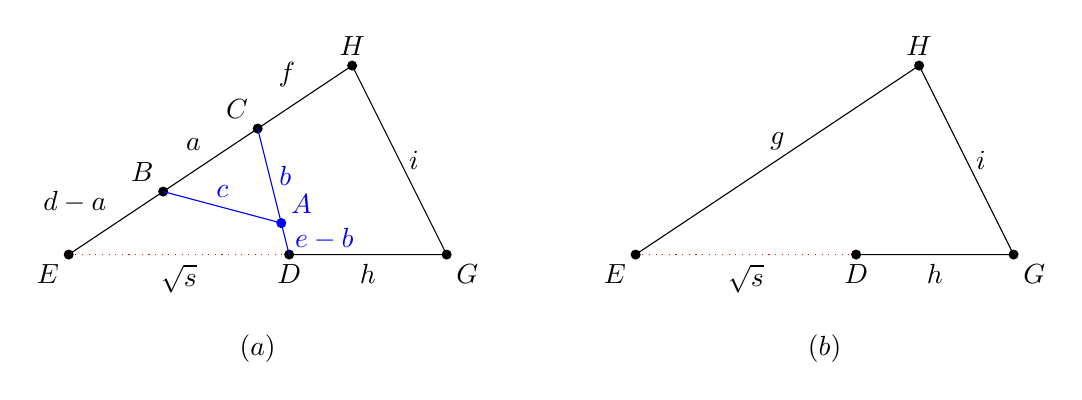
\begin{tikzpicture}
\begin{scope}[scale=0.4]
\begin{scope}
\draw[red,dotted] (0,0) -- node[below,black]{$\sqrt{s}$}++(7,0);
\draw[black,fill=black] (7,0) node[below]{$D$}  circle(4pt)
-- node[below]{$h$} ++(5,0) node[below right]{$G$} circle(4pt)
-- node[right]{$i$} ++(-3,6) node[above]{$H$} circle(4pt)
-- node[above left]{$f$} ++(-3,-2) node[above left]{$C$} circle(4pt)
-- node[above left]{$a$} ++(-3,-2) node[above left]{$B$} circle(4pt)
-- node[above left]{$d-a$} ++(-3,-2) node[below left]{$E$} circle(4pt);
\draw[blue,fill=blue] (7,0)
-- node[right]{$e-b$} ++(-.25,1) node[above right]{$A$} circle(4pt)
-- node[right]{$b$} ++(-.75,3)
   ++(+.75,-3)
-- node[above]{$c$} (3,2);
\draw[black](6,-3) node{$(a)$};
\end{scope}

\begin{scope}[shift={(18,0)}]
\draw[red,dotted] (0,0) -- node[below,black]{$\sqrt{s}$}++(7,0);
\draw[black,fill=black] (7,0) node[below]{$D$}  circle(4pt)
-- node[below]{$h$} ++(5,0) node[below right]{$G$} circle(4pt)
-- node[right]{$i$} ++(-3,6) node[above]{$H$} circle(4pt)
-- node[above]{$g$} ++(-9,-6) node[below left]{$E$} circle(4pt);
\draw[black](6,-3) node{$(b)$};
\end{scope}


\end{scope}
\end{tikzpicture}
\caption{The five strips intented to form an algebraic distance $\overline{EG} = \sqrt{s} + h$.}
\label{fig:alg-not-right}
\end{figure}

From figure \ref{fig:alg-not-right} $(a)$ we know $\sqrt{s}$ distance
between nodes $E$ and $D$ is produced by the three strips frame $a+d$, $b+e$ and $c$.
Using the law of cosines we calculate the angle $\theta = \angle{CED}$ in terms of $\sqrt{s}$:

\begin{align}
\cos\theta &= \frac{d^2 + (\sqrt{s})^2 - e^2}{2d\sqrt{s}} \nonumber\\
 &= \frac{(d^2 + s - e^2)\sqrt{s}}{2ds} \\
 &= \frac{m\sqrt{s}}{n} \label{eq:cos1}\\
 m &= d^2 + s - e^2 \\
 n &= 2ds
\end{align}

From figure \ref{fig:alg-not-right} $(a)$ we notice two sets of points are collinear:
$\{ E,B,C,H \}$ and $\{ E,D,G \}$. Using the law of cosines we calculate the 
angle $\theta = \angle{HEG}$ in terms of distances $g,\sqrt{s}+h,i$:

\begin{align}
\cos\theta &= \frac{g^2 + (\sqrt{s}+h)^2 - i^2}{2g(\sqrt{s}+h)} \nonumber\\
 &= \frac{g^2 + s + 2\sqrt{s}h + h^2 - i^2}{2g(\sqrt{s}+h)} \nonumber\\
 &= \frac{g^2 + s + h^2 - i^2+ 2\sqrt{s}h}{2g(\sqrt{s}+h)}
\end{align}

We multiply both numerator and denominator by $\sqrt{s}-h$ to eliminate the surd from denominator:
\begin{align}
\cos\theta &= \frac{(s + g^2 + h^2 - i^2)(\sqrt{s}-h) + 2\sqrt{s}h(\sqrt{s}-h)}
	{2g(\sqrt{s}+h)(\sqrt{s}-h)} \nonumber\\
 &= \frac{(s + g^2 + h^2 - i^2)(\sqrt{s}-h) + 2sh - 2\sqrt{s}h^2}
	{2g(s-h^2)} \nonumber\\ 
 &= \frac{-h(s + g^2 + h^2 - i^2 - 2s) + (s + g^2 + h^2 - i^2 - 2h^2)\sqrt{s}}
	{2g(s-h^2)} \nonumber\\ 
 &= \frac{h(s - g^2 - h^2 + i^2) + (s + g^2 - h^2 - i^2)\sqrt{s}}
	{2g(s-h^2)} \nonumber\\ 
 &= \frac{o + p\sqrt{s}}{q} \label{eq:cos2}\\
o &= h(s - g^2 - h^2 + i^2) \\
p &= s + g^2 - h^2 - i^2 \\
q &= 2g(s-h^2)
\end{align}

We compare both cosines equations \ref{eq:cos1} and \ref{eq:cos2}:
\begin{align}
\frac{m\sqrt{s}}{n} &= \frac{o + p\sqrt{s}}{q}
\end{align}
Since all variables are integers we need two conditions. First $o$ should be zero.
And second $\frac{m}{n} = \frac{p}{q}$.

For condition 1, we force $o$ to be zero:
\begin{align}
o &= 0 \nonumber\\
h(s - g^2 - h^2 + i^2) & = 0 \nonumber\\
s &= g^2 + h^2 - i^2 \label{eq:condition1}
\end{align}

For condition2, we force $m,n,p,q$ as:
\begin{align}
\frac{m}{n} &= \frac{p}{q} \nonumber\\
\frac{d^2 + s - e^2}{2ds} &= \frac{s + g^2 - h^2 - i^2}{2g(s-h^2)} \nonumber\\
\end{align}

We replace the value of $s$ of last equation RHS with the value of equation \ref{eq:condition1}
of condition 1:
\begin{align}
\frac{d^2 - e^2 + s}{ds} &= \frac{s + g^2 - h^2 - i^2}{g(s-h^2)} \nonumber\\
 &= \frac{g^2 + h^2 - i^2 + g^2 - h^2 - i^2}{g(g^2 + h^2 - i^2-h^2)} \nonumber\\
 &= \frac{2(g^2 - i^2)}{g(g^2 - i^2)} \nonumber\\
 &= \frac{2}{g} \nonumber\\
(d^2 - e^2 + s)g &= 2ds \label{eq:condition2}
\end{align}

\boxed{TODO: Examples!!!}



\section{Triangle pair frame}

\begin{figure}[H]
\centering
\begin{center}
\meccanoframetrianglepair{2}{3}{4} {3}{5}{7} {3pt}{1.0}{7}
\end{center}
\caption{Triangle pair frame.}
\label{fig:tripair}
\end{figure}

Figure \ref{fig:tripair} shows a triangle pair frame.
The pair joins triangles $\triangle{ABC}$ and $\triangle{DEF}$ in such a way vertices $C$ and $F$ coincide and vertices $A,C,D,F$ be collinear. With only five strips this frame is small and useful to make up the rigid polygons diagonals of the form
$g = \overline{BE} = \dfrac{z_2\sqrt{z_3+z_4\sqrt{z_5}}}{z_1}, z_i \in \bbb{Z}$. In some cases the diagonal can be denested to the form $g = \dfrac{z_2 + z_3\sqrt{z_4}}{z_1}$.

\subsection{Triangle pair algebra}

Using the law of cosines we calculate the angle $\theta = \angle{ACB}$ with defined variables $m,n$ and the angle $\phi = \angle{DFE}$ with defined variables $o,p$:
\begin{align}
(\theta, m, n) &\equiv (\angle{ACB}, a^2 + b^2 - c^2, 2ab), \quad | m | \le n, \quad m,n \in \bbb{Z} \label{eq:mn}\\
\cos\theta &= \frac{m}n \\
\sin\theta &= \sqrt{1-\cos^2\theta} = \frac{\sqrt{n^2 - m^2}}n \\
(\phi, o, p) &\equiv (\angle{DFE}, d^2 + e^2 - f^2, 2de), \quad | o | \le p, \quad o,p \in \bbb{Z} \label{eq:op}\\
\cos\phi   &= \frac{o}p \\
\sin\phi   &= \sqrt{1-\cos^2\phi} = \frac{\sqrt{p^2 - o^2}}p
\end{align}

Then, we use the cosines sum identity:
\begin{align}
\cos(\theta+\phi) &= \cos\theta\cos\phi - \sin\theta\sin\phi \nonumber\\
 &= \left(\frac{m}n\right)\left(\frac{o}p\right)
  - \left(\frac{\sqrt{n^2 - m^2}}n\right)\left(\frac{\sqrt{p^2 - o^2}}p\right) \nonumber\\
 &= \frac{mo - \sqrt{(n^2 - m^2)(p^2 - o^2)}}{np}
\end{align}

Finally we can calculate the distance $g \equiv \overline{BE}$ using the law of cosines:
\begin{align}
g &\equiv \overline{BE}\nonumber\\
 &= \sqrt{a^2 + d^2 - 2ad\cos(\theta+\phi)}\nonumber\\
 &= \sqrt{a^2 + d^2 - 2ad\left(\frac{mo - \sqrt{(n^2 - m^2)(p^2 - o^2)}}{np}\right)}\nonumber\\
 &= \sqrt{a^2 + d^2 - 2ad\left(\frac{mo - \sqrt{(n^2 - m^2)(p^2 - o^2)}}{4abde}\right)}\nonumber\\
 &= \sqrt{a^2 + d^2 - \frac{mo - \sqrt{(n^2 - m^2)(p^2 - o^2)}}{2be}}\nonumber\\
 &= \frac{\sqrt{4b^2e^2(a^2 + d^2) - 2bemo + 2be\sqrt{(n^2 - m^2)(p^2 - o^2)}}}{2be}
\end{align}

\subsection{Triangle pairs software}

From the last equation of $g$ we identify three \texttt{input} integers $i_1,i_2,i_3$ which are used to get $g(i)$. Then the nested radicals sofware will return square-free \texttt{output} integers $z_1,z_2,z_3,z_4,z_5$ as $g(z)$:
\begin{align}
i_1 &\equiv 2be\\
i_2 &\equiv i_1^2(a^2+d^2) - i_1mo\\
i_3 &\equiv (n^2-m^2)(p^2-o^2)\\
g(i) &= \frac{\sqrt{i_2 + i_1\sqrt{i_3}}}{i_1}\\
g(z) &= \frac{z_2\sqrt{z_3 + z_4\sqrt{z_5}}}{z_1}
\end{align}

We run a program to print a list of triangle pairs with sides $1 < a,b,c,d,e,f \leq max$ having a given distance $\overline{BE}=g$ or particular $z3,z4,z5$. Next example request a pairs list with $g = z_2\sqrt{46+18\sqrt{5}}/z_1$ up to strip length $10$ so we set as limits $max=10, z_3=46, z_4=18, z_5=5$ to get next report (text in blue):

\begin{MyColorPar}{blue}
%%----------- start
\begin{align*}
Folder &: \texttt{github.com/heptagons/meccano/frames}\\
Call &: \texttt{NewFrames().TrianglePairsTex(10, [46 18 5])}\end{align*}
\begin{align*}
(a,b,c) \oplus (d,e,f) &\mapsto g\\
\hline
%a=1...\\ 
%a=2...\\ 
(2,1,2) \oplus (3,3,3) &\mapsto \frac{\sqrt{46+18\sqrt{5}}}{2} \\
(2,1,2) \oplus (3,8,7) &\mapsto \frac{\sqrt{46+18\sqrt{5}}}{2} \\
(2,2,2) \oplus (3,6,6) &\mapsto \frac{\sqrt{46+18\sqrt{5}}}{2} \\
(2,3,4) \oplus (3,5,7) &\mapsto \frac{\sqrt{46+18\sqrt{5}}}{2} \\
(2,4,4) \oplus (3,8,7) &\mapsto \frac{\sqrt{46+18\sqrt{5}}}{2} \\
%a=3...\\ 
(3,3,3) \oplus (2,4,4) &\mapsto \frac{\sqrt{46+18\sqrt{5}}}{2} \\
%a=4...\\ 
(4,2,4) \oplus (6,6,6) &\mapsto \sqrt{46+18\sqrt{5}} \\
(4,4,4) \oplus (6,7,8) &\mapsto \sqrt{46+18\sqrt{5}} \\
%a=5...\\ 
%a=6...\\ 
(6,3,6) \oplus (4,4,4) &\mapsto \sqrt{46+18\sqrt{5}} \\
(6,3,6) \oplus (9,9,9) &\mapsto \frac{3\sqrt{46+18\sqrt{5}}}{2} \\
(6,6,6) \oplus (4,8,8) &\mapsto \sqrt{46+18\sqrt{5}} \\
(6,7,8) \oplus (9,9,9) &\mapsto \frac{3\sqrt{46+18\sqrt{5}}}{2} \\
%a=7...\\ 
%a=8...\\ 
%a=9...\\ 
%a=10...\\ 
\end{align*}
%%----------- end
\end{MyColorPar}

\begin{figure}[H]
\centering
\begin{center}
\meccanoframetrianglepair{2}{1}{2} {3}{3}{3} {3pt}{1.0}{3} % last 3 is to show vertices/sides
\end{center}
\caption{Triangle pair frame $(2,1,2) \oplus (3,3,3)$ makes $\overline{BE} = \dfrac{\sqrt{46+18\sqrt{5}}}{2}$.}
\label{fig:tripair212333}
\end{figure}

In figure \ref{fig:tripair212333} we build a triangular pair following one of the last report results, when $abc=(2,1,2)$ and $def=(3,3,3)$.

%%%%%%%%%

\section{Triangle pair extended frame}

\begin{figure}[H]
 \centering
 \begin{tikzpicture}
  \begin{scope}[scale=0.50]
   \begin{scope}[shift={(0,0)}]
    \meccanoframetrianglex{0}{4}{5}{6} {0}{0}{3pt} 
    \meccanoframetrianglex{1}{3}{3}{2} {0}{0}{3pt}
    \draw (2.5,-5) node{$(a)$};
   \end{scope}
   \begin{scope}[shift={(8,0)}]
    \meccanoframetrianglex{0}{4}{5}{6} {7}{0}{3pt}
    \meccanoframetrianglex{1}{3}{3}{2} {4}{0}{3pt}
    \draw (3.5,-5) node{$(b)$};
   \end{scope}
   \begin{scope}[shift={(18,0)}]
    \meccanoframetrianglex{0}{4}{5}{6} {7}{1}{3pt}
    \meccanoframetrianglex{1}{3}{3}{2} {4}{1}{3pt}
    \draw (3.5,-5) node{$(c)$};
   \end{scope}
   \begin{scope}[shift={(28,0)}]
    \meccanoframetrianglex{0}{4}{5}{6} {7}{-3}{3pt}
    \meccanoframetrianglex{1}{3}{3}{2} {4}{-2}{3pt}
    \draw (3.5,-5) node{$(d)$};
   \end{scope}
  \end{scope}
 \end{tikzpicture}
 \caption{Triangle pair extended frame. Starts like previous triangle pair frame except
 we can extend strips $\alpha$ or $\gamma$, $\delta$ or $\zeta$, and we can separate vertices $C$ and $F'$.
 Vertices $A,C,D',F'$ remain collinear and we are interested in the distance $g \equiv \overline{B'E'}$. We show four examples: (a) is the original triangle pair,
 (b) has moved the $\triangle{D'E'F'}$ to the right,
 (c) also extends strips $\alpha$ and $\delta$ and (d) extends strips $\gamma$ and $\zeta$.
 }
 \label{fig:tripairext}
\end{figure}

We show some triangle pair extended frames in figure \ref{fig:tripairext}.
As with not-extended triangle pair of figure \ref{fig:tripair} we also have two triangles with five strips, but we can perform one, two or three transformations on the frame: 
\begin{enumerate}
 \item Separate nodes $C$ and $F$ which moves $\triangle{D'E'F'}$.
 \item Extends strip $a \rightarrow \alpha$ or strip $c \rightarrow \gamma$ but not both.
 \item Extend strip $d \rightarrow \delta$ or strip $f \rightarrow \zeta$ but not both.
\end{enumerate}

For each transformation we define three integers $x, y_1, y_2$:
\begin{align}
x &= \left \{ \begin{array}{rl}
 0       &  C,F \mbox{ vertices remain joined}\\
 \geq  0 &  \triangle{DEF} \mbox{ is moved to the right a distance equal to } x \\
 \end{array}\right. \\
y_1 &= \left \{ \begin{array}{rl}
 0   & \alpha = a,\quad \gamma = c \\
 > 0 & \alpha = a + y_1,\quad \gamma = c \\
 < 0 & \alpha = a,\quad \gamma = c + |y_1| \\
 \end{array}\right. \\ 
y_2 &= \left \{ \begin{array}{rl}
 0   & \delta = d,\quad \zeta = f \\
 > 0 & \delta = d + y_2,\quad \zeta = f \\
 < 0 & \delta = d,\quad \zeta = f + |y_2| \\
 \end{array}\right. 
\end{align}

Let define $M(a,b,c)$ the triangle above, $N(d,e,f)$ the triangle below and $T(x,y_1,y_2)$ the transformations.
Then we can describe the cases $(a)-(d)$ of figure \ref{fig:tripairext} as operations:
\begin{align*}
(a) &: M(4,5,6) \oplus N(4,4,2) \oplus T(0,0,0) \\
(b) &: M(4,5,6) \oplus N(4,4,2) \oplus T(4,0,0) \\
(c) &: M(4,5,6) \oplus N(4,4,2) \oplus T(4,+2,+1) \\
(d) &: M(4,5,6) \oplus N(4,4,2) \oplus T(4,-3,-2)
\end{align*}

\subsection{Triangle pair extended frame algebra}

We are going to calculate the diagonal $g \equiv \overline{B'E'}$ of the triangle pair extended using the $M,N,T$ values. We start setting the vertex $C$ at the origin of the standard two-dimensional graph and defining $(B_x, By)$ the abscissa and ordinate of vertex $B'$ and
$(E_x, E_y)$ the abscissa and ordinate of vertex $E'$.

For the triangle above $M(a,b,c)$ we have two cases: $T(0,y_1 \geq 0,0)$ and $T(0,y_1 < 0,0)$.
In the not-extended triangle pair we already calculated $\theta=\angle{ACB}, \cos\theta, \sin\theta$ based in $m,n$ of equation \ref{eq:mn}.
For the case $y_1 < 0$ here, we calculate also $\omega=\angle{BAC},\cos\omega,\sin\omega$ using two variables $p,q$. For both cases we define $u = |y_1|$ and finally we get $(B_x, B_y)$:
\begin{align}
(\omega, p, q) &\equiv (\angle{BAC}, b^2 + c^2 - a^2, 2bc), \quad | p | \le q, \quad p,q \in \bbb{Z} \label{eq:pq}\\
\cos\omega &= \frac{p}q \\
\sin\omega &= \sqrt{1-\cos^2\omega} = \frac{\sqrt{q^2 - p^2}}q \\
\alpha &= a + u\\
\gamma &= c + u\\
B_x &= \left \{ \begin{array}{rl}
  y_1 \geq 0 & \alpha\cos\theta\\
  y_1 < 0    & b - \gamma\cos\omega
 \end{array}\right. \\
B_y &= \left \{ \begin{array}{rl}
 y_1 \geq 0 & \alpha\sin\theta\\
 y_1 < 0    & \gamma\sin\omega
 \end{array}\right.
\end{align}

For the triangle below $N(d,e,f)$ we have two cases: $T(x,0,y_2 \geq 0)$ and $T(x,0,y_2 < 0)$. In both cases we will use $x \geq 0$ always for simplicity.
In the not-extended triangle pair we already calculated $\phi=\angle{DFE}, \cos\phi, \sin\phi$
defining $o,p$ in equation \ref{eq:op}.
For the case $y_2 < 0$ here we calculate also $\psi=\angle{EDF}, \cos\psi, \sin\psi$ using two variables $r,s$. For both cases we define $v = |y_2|$ and finally we get $(E_x,E_y)$:
\begin{align}
(\psi, r, s) &\equiv (\angle{EDF}, e^2 + f^2 - d^2, 2ef), \quad | r | \le s, \quad r,s \in \bbb{Z} \label{eq:rs}\\
\cos\psi &= \frac{r}s \\
\sin\psi &= \sqrt{1-\cos^2\psi} = \frac{\sqrt{s^2 - r^2}}s \\
\delta &= d + v\\
\zeta  &= f + v\\
E_x &= \left \{ \begin{array}{rl}
 y_2 \geq 0 & x + \delta\cos\phi\\
 y_2 < 0    & x + e - \zeta\cos\psi 
 \end{array}\right. \\
E_y &= \left \{ \begin{array}{rl}
 y_2 \geq 0 & -\delta\sin\phi \\
 y_2 < 0    & -\zeta\sin\psi
 \end{array}\right.
\end{align}

With the four components $B_x, B_y, E_x, E_y$ we can calculate $g = \overline{B'E'}$:
\begin{align}
g &= \sqrt{(B_x + E_x)^2 + (B_y + E_y)^2} \\
 &= \sqrt{(B_x^2 + B_y^2) + (E_x^2 + E_y^2) + 2B_xE_x + 2B_yE_y} \label{eq:tpeg}
\end{align}

We need to calculate separated four types of diagonals $g^{++},g^{+-},g^{-+},g^{--}$ according the signs of $y_1$ and $y_2$ as described in the next table:
\begin{center}
\begin{tabular}{| c c c |}
\hline
$g$ & $y_1$ & $y_2$ \\ [0.5ex]
\hline
$g^{++}$ & $\geq 0$ & $\geq 0$ \\
$g^{+-}$ & $\geq 0$ & $< 0$ \\
$g^{-+}$ & $< 0$ & $\geq 0$ \\
$g^{--}$ & $< 0$ & $< 0$ \\
\hline
\end{tabular}
\end{center}

\subsection{Triangle pair extended case $g^{++}$ ($y_1\geq 0$ and $y_2\geq 0$)}

For $g^{++}$ we calculate sums and products of $Bx,By,Ex,Ey$ when $y_1 \geq 0$ and $y_2 \geq 0$:
\begin{align}
\alpha &= a + u, \qquad \delta = d + v\\
(B_x^2 + B_y^2)^{++} &= \alpha^2\cos^2\theta + \alpha^2\sin^2\theta \nonumber\\
 &= \alpha^2\\
(E_x^2 + E_y^2)^{++} &= (x + \delta\cos\phi)^2 + (-\delta\sin\phi)^2 \nonumber\\
 &= x^2 + 2x\delta\cos\phi + \delta^2\cos^2\phi + \delta^2\sin^2\phi \nonumber\\
 &= x^2 + 2x\delta\cos\phi + \delta^2 \nonumber\\
 &= \frac{px^2 + 2x\delta o + p\delta^2}{p}\\
(B_xE_x)^{++} &= (\alpha\cos\theta)(x + \delta\cos\phi) \nonumber\\
 &= \frac{\alpha m(px + \delta o)}{np} \\
(B_yE_y)^{++} &= (\alpha\sin\theta)(-\delta\sin\phi)\nonumber\\
 &= -\frac{\alpha \delta\sqrt{(n^2 - m^2)(p^2 - o^2)}}{np}
\end{align}
We subsitute the products in equation \ref{eq:tpeg}:
\begin{align}
g^{++} &= \sqrt{(B_x^2 + B_y^2)^{++} + (E_x^2 + E_y^2)^{++} + 2(B_xE_x)^{++} + 2(B_yE_y)^{++}}\nonumber\\
 &= \sqrt{
\alpha^2
+ \frac{px^2 + 2x\delta o + p\delta^2}p
+ \frac{2\alpha m(px + \delta o)}{np}
- \frac{2\alpha \delta\sqrt{(n^2 - m^2)(p^2 - o^2)}}{np}
}\nonumber\\
 &= \frac{\sqrt{
n^2p^2\alpha^2 + n^2p(px^2 + 2x\delta o + p\delta^2)
+ 2\alpha mnp(px + \delta o) - 2\alpha\delta np\sqrt{(n^2 - m^2)(p^2 - o^2)}
}}{np}
\end{align}

From the last equation we identify four \texttt{input} integer variables to calculate software $g^{++}(i)$ which will be reduced or even denested $g^{++}(z)$:
\begin{align}
i_1 &= np \\
i_2 &= i_1^2\alpha^2 + i_1n(px^2 + 2x\delta o + p\delta^2) + 2\alpha mi_1(px + \delta o)\\
i_3 &= - 2\alpha\delta i_1 \nonumber\\
i_4 &= (n^2 - m^2)(p^2 - o^2)\\
g^{++}(i) &= \frac{\sqrt{i_2 + i_3\sqrt{i_4}}}{i_1}\\
g^{++}(z) &= \frac{z_2\sqrt{z_3 + z_4\sqrt{z_5}}}{z_1}
\end{align}



%\section{Two triangles with offsets}
%
%\begin{figure}[H]
%\centering
%\begin{center}
%% a,b,c,d,e,p,scale, x+g, g,h,i,j,k, x,p
%\meccanoframefive{6}{5}{5}{3}{2}{3pt}{0.6} {7} {3}{4}{4}{3}{2} {3} (a)
%\meccanoframefive{6}{5}{5}{0}{2}{3pt}{0.7} {7} {3}{4}{4}{0}{2} {3} (b)
%\end{center}
%\caption{Frame of two triangles with offsets. We construct two triangles $\triangle{ABC}$ and
%$\triangle{GHI}$. Extending the strips we get four vertices $E,D,J,K$ which
%can form four rigid distances of surd type: $\overline{DJ}, \overline{DK},
%\overline{EJ}, \overline{EK}$.}
%\label{fig:5strips}
%\end{figure}
%
%Figure \ref{fig:5strips} shows a frame with five strips. The frame has eleven variables:
%\begin{align}
%a &= \overline{BC}, \quad b = \overline{AC}, \quad c = \overline{AB}\\
%d &= \overline{AE}, \quad e = \overline{AD}\\
%f &= \overline{AG}\\
%g &= \overline{HI}, \quad h = \overline{GI}, \quad i = \overline{GH}\\
%j &= \overline{HJ}, \quad k = \overline{HK}
%\end{align}
%
%Assume vertex A is at the origin.
%Let $\alpha = \angle{BAC}$, and $D_x,D_y$ the abscissa and orditate of vertex $D$ so we have:
%\begin{align}
%t &\equiv b^2 + c^2 - a^2\\
%x &\equiv 4b^2c^2 - t^2\\
%\cos\alpha &= \frac{t}{2bc}\\
%\sin\alpha &= \frac{\sqrt{x}}{2bc}\\
%D_x &= d\sin\alpha = \frac{d\sqrt{x}}{2bc}\\
%D_y &= d\cos\alpha = \frac{dt}{2bc}\\
%D_x^2 + D_y^2 &= d^2
%\end{align}
%Let $\delta = \angle{HGI}$ and $K_x,K_y$ the abscissa and ordinate of
%vertex $K$ so we have:
%\begin{align}
%v &\equiv h^2 + i^2 - g^2\\
%y &\equiv 4h^2i^2 - v^2\\
%\cos\delta &= \frac{v}{2hi}\\
%\sin\delta &= \frac{\sqrt{y}}{2hi}\\
%K_x &= f + k\sin\delta = f + \frac{k\sqrt{y}}{2hi}\\
%K_y &= -k\cos\delta = -\frac{kv}{2hi}\\
%K_x^2 + K_y^2 &= f^2 + 2fk\sin\delta + k^2\\
% &= f^2+k^2 + \frac{fk\sqrt{y}}{hi}
%\end{align}
%We calculate the distance $\overline{DK}$:
%\begin{align}
%\overline{DK}^2 &= (D_x+K_x)^2 + (D_y+K_y)^2 \nonumber\\
% &= D_x^2 + 2D_xK_x + K_x^2 + D_y^2 + 2D_yK_y + K_y^2 \nonumber\\
% &= (D_x^2+D_y^2) + (K_x^2+K_y^2) + 2D_xK_x + 2D_yK_y \nonumber\\
% &= d^2 + f^2 + k^2 + \frac{fk\sqrt{y}}{hi}
%  + 2\left(\frac{d\sqrt{x}}{2bc}\right)\left(f + \frac{k\sqrt{y}}{2hi}\right)
%  + 2\left(\frac{dt}{2bc}\right)\left(-\frac{kv}{2hi}\right) \nonumber\\
% &= d^2 + f^2 + k^2 - \frac{dtkv}{2bchi} + \frac{fk\sqrt{y}}{hi}
%  + \frac{df\sqrt{x}}{bc} + \frac{dk\sqrt{xy}}{2bchi}
%\end{align}

\end{document}